\chapter{Solution Design}
\label{sec:solution}

\section{Requirements}
\label{sec:solution:req}
\subsection{Functional Requirements}
The system must meet the following core requirements for a MVP:\\
It shall integrate the necessary modeling functionalities within one unified interface (webpage).\\
It shall support upload multiple documents in textual format, e.g.,TXT, DOCX, PDF.\\
It shall allow users to select multiple passages from one document to serve as input for LLM-based process model auto-generation. \\
It shall provide a clear visual link between the text and the generated model.\\
It shall allow users to establish process-subprocess relationships between models.\\
It shall record user behavior and interactions with the system for analysis purposes.\\
One additional requirement is that the system shall be able to support document update.
\subsection{Non-functional Requirements}
Non-functional requirements for this tool mainly regard technical constraints:\\
It shall be implemented as a web-based application.\\
The frontend shall be developed using native web technologies (JavaScript, HTML, and CSS).\\
The visualization of the process model shall be implemented using the CPEE Layout\footnote{\url{https://github.com/etm/cpee-layout}} library.\\
The source text for the process model should be embedded in the model's XML data.\\
The LLM-backed process model generation shall be implemented using the API from AutoBPMN.AI.\\

\section{System Overview}
Since the innovation of this tool focuses on the integration of functionalities and an innovative modeling workflow in the frontend, so the system overview is described from the user perspective, which is the frontend part of the system.

Firstly, we define the following concepts to better describe the system overview:\\
- Project: one use case or one task that the user wants to accomplish, which may involve multiple documents that models needs to be created from. \\
- Workspace: the unfied page for one project, where the entire modeling workflow can be accomplish from document upload to model export.\\
- Traceability: the ability to find the source text on the document for a model and the ability to find the model on the source text from documents.\\
- Project graph: a network-style visualization of the relationships between different models within a project, which can help users to understand the overall structure and flow of the processes being modeled. Details can be found in the section.

It contains three pages: a home page where a user can create a new project or open an existing project, a workspace page where the modeling workflow happens, and a statistic page where the user can view the statistics of the project. 
\section{Modeling Workflow Design}
As the core part of the system, this section describes the modeling workflow that happens in the workspace page in Use Case Diagram.
Figure: the use case diagram for the interaction of a user within the workspace page.\\
user --> Upload/Rename/Update/Delete Document\\
     --> View document --> Select Text Passages --> Generate Process Model\\
     --> View Process Model --> Modify Process Model --> Link Process Model with other Models\\
     --> Rename/Delete/Export Process Model
\section{Core Functionalities Design}
\subsection{Document Management}

\subsection{Document Interaction}
text selection
text selection editing
\subsection{Process modeling}

\subsubsection{Human-in-the-loop Process Modeling and Version Control}

\subsubsection{Use Case: Model Generation}
By click the button an adavance mode is desgin 
\subsubsection{Use Case: Model Modification}
a. Manual edit
b. Update selected text and apply the changes. 
c. Refinement by sending prompt to LLM:\\
   Input: prompt only and the current Model\\
d. Regeneration:\\
   Input: type a. current model + changed selected text passage b. advanced mode: prompt + current model + changed selected text passage
   
\subsubsection{Use Case: Establishing Process-Subprocess Relationships}

- a review step for each LLM-generated model.
\subsubsection{Augumented Model Data}


\begin{figure}[H]
  \centering
  \caption{Example JSON schema used in the backend for text quotes}
  \label{fig:imp_backend_schema_example}
  \begin{lstlisting}[language=XML]
<textQuoteSelector>
</textQuoteSelector>
  \end{lstlisting}
\end{figure}


\subsection{Traceability}
It is a 
\subsection{Project Graph Visualization}
Visualize the 

\section{User Interface and Interaction Design}
The layout design of the user interface is shown in the figure~\ref{fig:sol_ui} in a 3-pane layout. The left pane is for document uploading and viewing, the middle pane is for process modeling and the right pane is for process models viewing and project graph visualization. The details are divided as the following: a) Document List b) Document Viewer c) Model Editor c.1) Model Canvas c.2) Model Prompt Editor d) Model List e) Project Graph Visualization.
Interacion Design:
The workspace support a highly freely interaction/navigation between model and documents.\\
A model can be triggered to be displayed by the following pathes:\\
(1). Click on the model in the model list\\
(2). Click on the text passage that is linked to the model\\
(3). Click on the model tag displayed above the text passage \\
(4). Click on the model node in the project graph visualization\\
A document can be triggered to be displayed by the following pathes:\\
(1). Click on the document in the document list\\
(2). Click on the model in the model list, then its corresponding document will be displayed and the linked text passage's position will be auto-anchored.\\
(3). Click on the document node in the project graph visualization\\

\section{System Architecture}
The system architecture is shown in the figure~\ref{fig:sol_architecture}. The system is designed as a web-based application, with a front-end implemented using native JavaScript, HTML, and CSS. The back-end is responsible for handling user interactions, managing document uploads, and communicating with the LLM API for process model generation. The visualization of the process models is achieved using the CPEE library, which allows for dynamic rendering of BPMN diagrams based on the generated models.
\begin{figure}[H]
    \centering
    \caption{System Architecture} 
    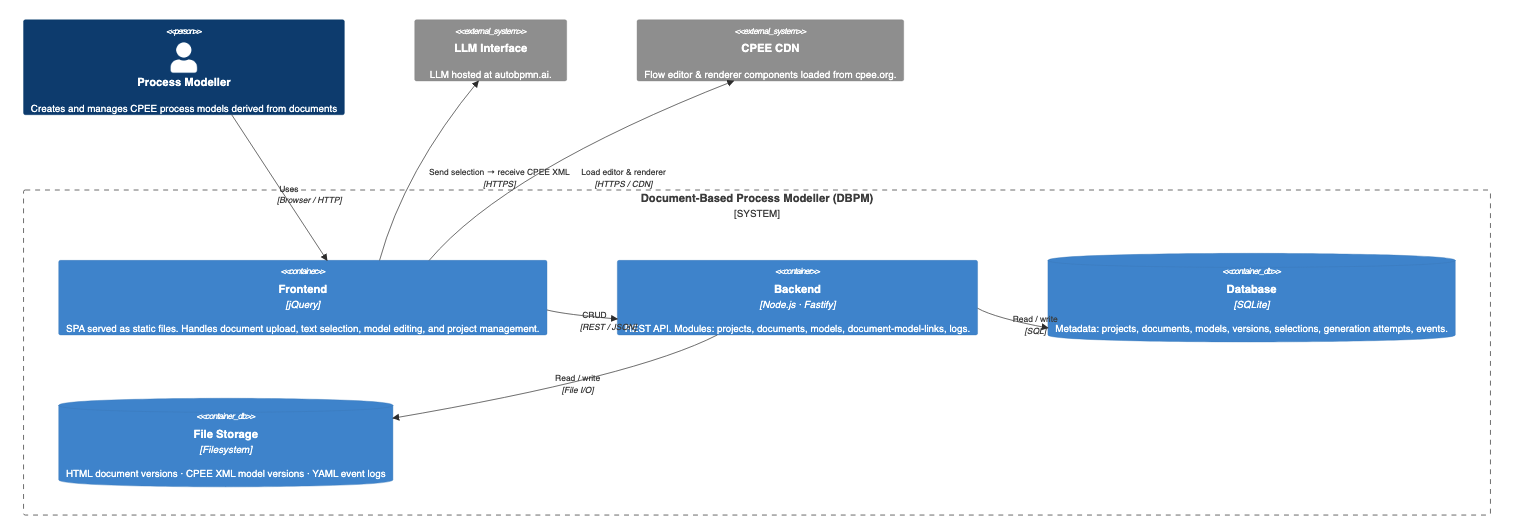
\includegraphics[width=0.8\textwidth]{images/sol_architecture.png}
    \floatfoot{The system architecture of the document-based process modeling tool.}
    \label{fig:sol_architecture}
\end{figure}

\section{Conceptual Data Model}
\begin{figure}[H]
    \centering
    \caption{Conceptual Data Model} 
    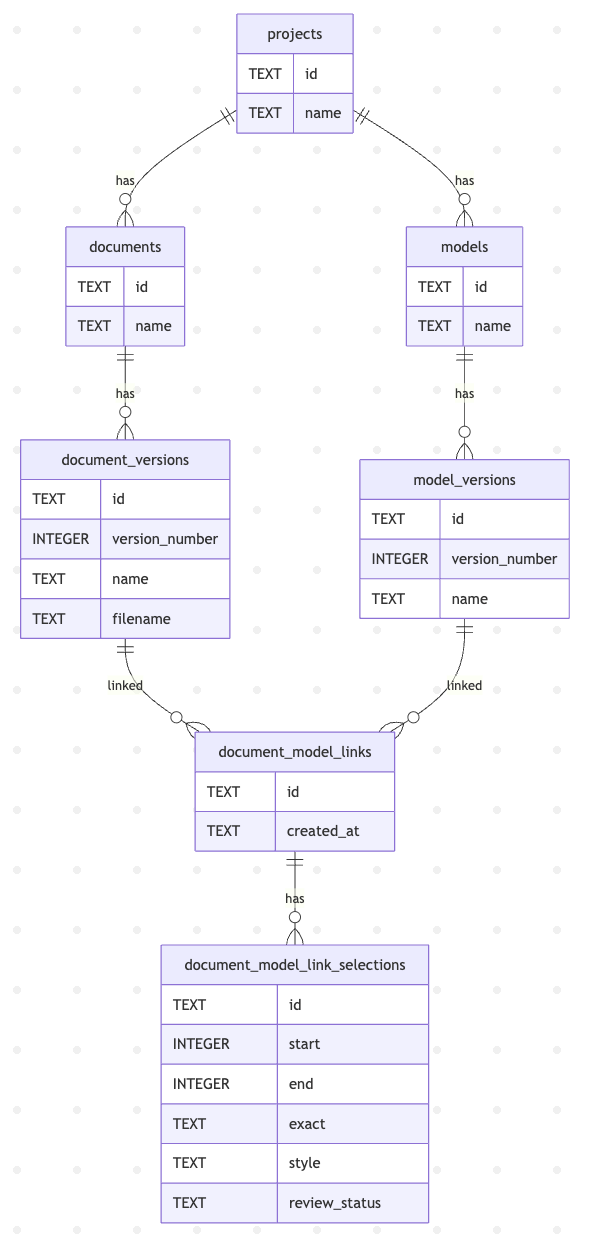
\includegraphics[width=0.8\textwidth]{images/sol_data_model.png}
    \floatfoot{The conceptual data model of the document-based process modeling tool.}
    \label{fig:sol_data_model}
\end{figure}


The system uses a TextQuoteSelector for robust anchoring, as defined in the W3C Web Annotation Model (Text Quote Selector section) \cite{w3c_annotation_model}.
